\section{Introduction}
\label{sec:intro}

The \dword{dune} is a next-generation, long-baseline neutrino oscillation experiment which will carry out a detailed study of neutrino mixing utilizing high-intensity \numu and \anumu beams measured over a long baseline.
\dword{dune} is designed to make significant contributions to the completion of the standard three-flavor picture by measuring all the parameters governing $\nu_1$--$\nu_3$ and $\nu_2$--$\nu_3$ mixing in a single experiment. Its main scientific goals are the definitive determination of the neutrino mass ordering, the definitive observation of \dword{cpv} for more than 50\% of possible true values of the charge-parity violating phase, \deltacp,  
and precise measurement of oscillation parameters, particularly \deltacp, \sinstt{13}, and the octant of $\theta_{23}$.
These measurements will help guide theory in understanding if there are new symmetries in the neutrino sector and whether there is a relationship between the generational structure of quarks and leptons~\cite{Qian:2015waa}. Observation of \dword{cpv} in neutrinos would be an important step in understanding the origin of the baryon asymmetry of the universe~\cite{Fukugita:1986hr, Davidson:2008bu}.

The \dword{dune} experiment will observe neutrinos from a high-power neutrino beam peaked at $\sim$2.5 GeV but with a broad range of neutrino energies, a \dword{nd} located at Fermi National Accelerator Laboratory, in Batavia, Illinois, USA, and a large \dword{lartpc} \dword{fd} located at the 4850 ft level of Sanford Underground Research Facility (SURF), in Lead, South Dakota, USA, 1285~km from the neutrino production point. The neutrino beam provided by \dword{lbnf}~\cite{Abi:2020wmh} is produced using protons from Fermilab's Main Injector, which are guided onto a graphite target, and a traditional horn-focusing system to select and focus particles produced in the target~\cite{Abi:2020evt}. The polarity of the focusing magnets can be reversed to produce a beam dominated by either muon neutrinos or muon antineutrinos. A highly capable \dword{nd} will constrain many systematic uncertainties for the oscillation analysis. The 40-kt (fiducial) \dword{fd} is composed of four 10 kt (fiducial) LArTPC modules~\cite{Acciarri:2016crz,Acciarri:2015uup,Acciarri:2016ooe}.
The deep underground location of the \dword{fd} reduces cosmogenic and atmospheric sources of background, which also provides sensitivity to nucleon decay and low-energy neutrino detection, for example, the possible observation of neutrinos from a core-collapse supernova~\cite{Abi:2020evt}.

The entire complement of neutrino oscillation experiments to date has measured five of the neutrino mixing parameters~\cite{Esteban:2018azc,deSalas:2017kay,Capozzi:2017yic}: the three mixing angles $\theta_{12}$, $\theta_{23}$, and $\theta_{13}$, and the two squared-mass differences $\Delta m^{2}_{21}$ and $|\Delta m^{2}_{31}|$, where $\Delta m^2_{ij} = m^2_{i} - m^{2}_{j}$ is the difference between the squares of the neutrino mass states in eV$^{2}$.
The neutrino mass ordering (i.e., the sign of $\Delta m^{2}_{31}$) is unknown, though recent results show a weak preference for the normal ordering~\cite{Abe:2018wpn,PhysRevD.97.072001,PhysRevLett.123.151803}.
The value of \deltacp is not well known, though neutrino oscillation data are beginning to provide some information on its value~\cite{Abe:2018wpn,Abe:2019vii}.

The oscillation probability of \numu $\rightarrow$ \nue through matter in the standard three-flavor model and a constant density approximation is, to first order~\cite{Nunokawa:2007qh}:
\begin{equation}
  \begin{aligned}
    P(\;\nu^{\bracketbar}_\mu \rightarrow \nu^{\bracketbar}_e) & \simeq \sin^2 \theta_{23} \sin^2 2 \theta_{13} 
    \frac{ \sin^2(\Delta_{31} - aL)}{(\Delta_{31}-aL)^2} \Delta_{31}^2 \\
    & + \sin 2 \theta_{23} \sin 2 \theta_{13} \sin 2 \theta_{12}\frac{ \sin(\Delta_{31} - aL)}{(\Delta_{31}-aL)} \Delta_{31} \\
    &\times \frac{\sin(aL)}{(aL)} \Delta_{21} \cos (\Delta_{31} \pm \deltacp) & \\
    & + \cos^2 \theta_{23} \sin^2 2 \theta_{12} \frac {\sin^2(aL)}{(aL)^2} \Delta_{21}^2,
  \end{aligned}
  \label{eqn:appprob}
\end{equation}
where
\begin{equation*}
  a = \pm \frac{G_{\mathrm{F}}N_e}{\sqrt{2}} \approx \pm\frac{1}{3500~\mathrm{km}}\left(\frac{\rho}{3.0~\mathrm{g/cm}^{3}}\right),
\end{equation*}
$G_{\mathrm{F}}$ is the Fermi constant, $N_e$ is the number density of electrons in the Earth's crust, $\Delta_{ij} = 1.267 \Delta m^2_{ij} L/E_\nu$, $L$ is the baseline in km, and $E_\nu$ is the neutrino energy in GeV. 
Both \deltacp and $a$ terms are positive for
$\nu_\mu \to \nu_e$ and negative for $\bar{\nu}_\mu \to \bar{\nu}_e$ oscillations; i.e.,
a neutrino-antineutrino asymmetry is introduced both by \dword{cpv} (\deltacp)
and the matter effect ($a$). The origin of the matter effect asymmetry 
is simply the presence of electrons and absence of positrons in the Earth~\cite{Wolfenstein:1977ue,Mikheev:1986gs}.
The (anti-)electron neutrino appearance probability
is shown in 
Figure~\ref{fig:oscprob} at the \dword{dune} baseline of \SI{1285}\km{} as a function of neutrino 
energy for several values of \deltacp.

\begin{figure}[htbp]
  \centering
  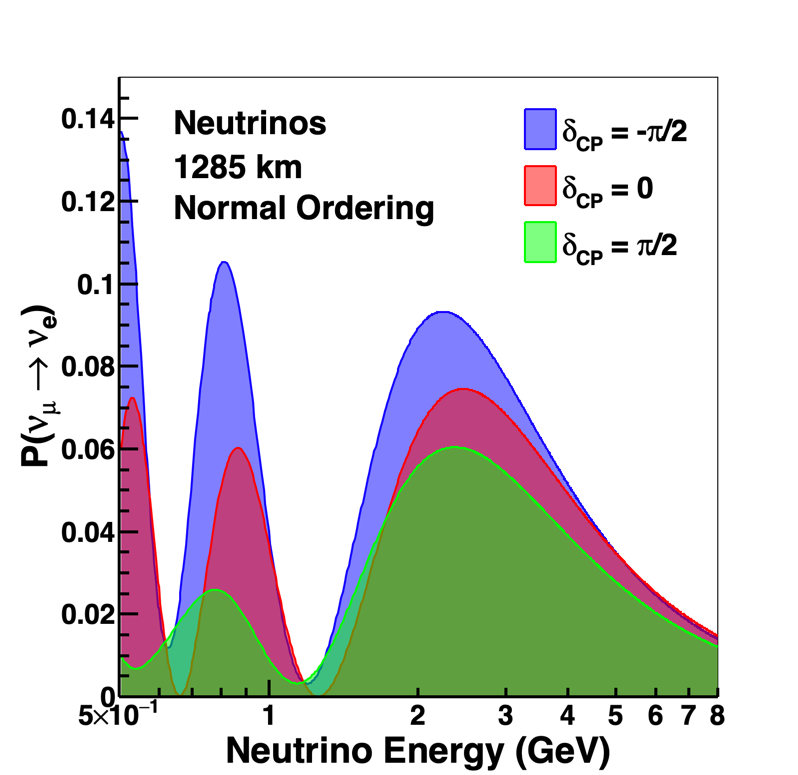
\includegraphics[width=0.98\linewidth]{DUNE_osc_prob_NH.png}\\
  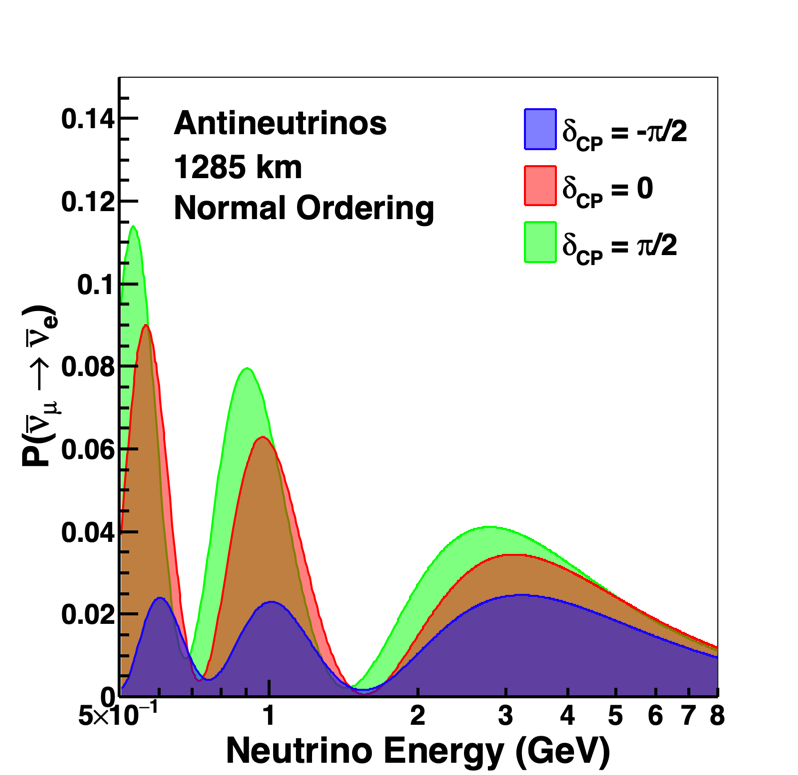
\includegraphics[width=0.98\linewidth]{DUNE_osc_prob_NH_anti.png}
  \caption[Appearance probabilities for \nue and \anue at \SI{1285}{\km}]{The appearance probability at a baseline of \SI{1285}\km{},
  as a function of neutrino energy, for \deltacp = $-\pi/2$ (blue), 
  0 (red), and $\pi/2$ (green), for neutrinos (top) and antineutrinos
  (bottom), for normal ordering.}
  \label{fig:oscprob}
\end{figure}

\dword{dune} has a number of features that give it unique physics reach, complementary to other existing and planned experiments~\cite{Ayres:2007tu,Abe:2011ks,Abe:2018uyc}. Its broad-band beam makes it sensitive to the shape of the oscillation spectrum for a range of neutrino energies. \dword{dune}'s relatively high energy neutrino beam enhances the size of the matter effect and will allow \dword{dune} to measure \deltacp and the mass ordering simultaneously. The unique \dword{lartpc} detector technology will enhance the resolution on \dword{dune}'s measurement of the value of \deltacp, and along with the increased neutrino energy, gives \dword{dune} a different set of systematic uncertainties to other experiments, making \dword{dune} complementary with them.

This paper describes studies that quantify DUNE's expected sensitivity to long-baseline neutrino oscillation, using the accelerator neutrino beam. Note that atmospheric neutrino samples would provide additional sensitivity to some of the same physics, but are not included in this work. The flux simulation and associated uncertainties are described in Section~\ref{sec:flux}. Section~\ref{sec:nuint} describes the neutrino interaction model and systematic variations. The near and far detector simulation, reconstruction, and event selections are described in Sections~\ref{sec:nd} and \ref{sec:fd}, respectively, with a nominal set of event rate predictions given in Section~\ref{sec:rate}. Detector uncertainties are described in Section~\ref{sec:syst}. The methods used to extract oscillation sensitivities are described in Section~\ref{sec:methods}. The primary sensitivity results are presented in Section~\ref{sec:sens}. We present our conclusions in Section~\ref{sec:conclude}.
